\graphicspath{{./images/CPN/}}
\chapter{Coloured Petri Nets}
\label{ch:CPN}
\paragraph*{\textnormal{Coloured Petri Net (CPN) is a graphical and formal modelling language used for modelling dynamic systems and analysing their properties. Modelling dynamic systems is a challenge in today's world. The reason for the same is that due to their complexity and property of concurrency and non-determinism, their execution path can be numerous. One simply cannot build the concurrent systems without proper analysis. The challenge is to build an executable model of the system. This will help in analysing systems and simulating them without actually building the real system. There are many application domains of CPNs which includes communication protocols, data networks, distributed algorithms, embedded systems etc. CPN, first introduced by Kurt Jensen, is an extension of Petri nets.}}

\subparagraph*{\textnormal{In this chapter, we start with a running example. Further, we explain the syntax of the modelling language and then we describe its execution semantics. All definitions in this chapter are taken from \cite{DBLP:books/daglib/CPN_Book}.}}

\section{Example} \label{sec:CPN_Example}
\begin{figure}[!htbp]
	\centering
	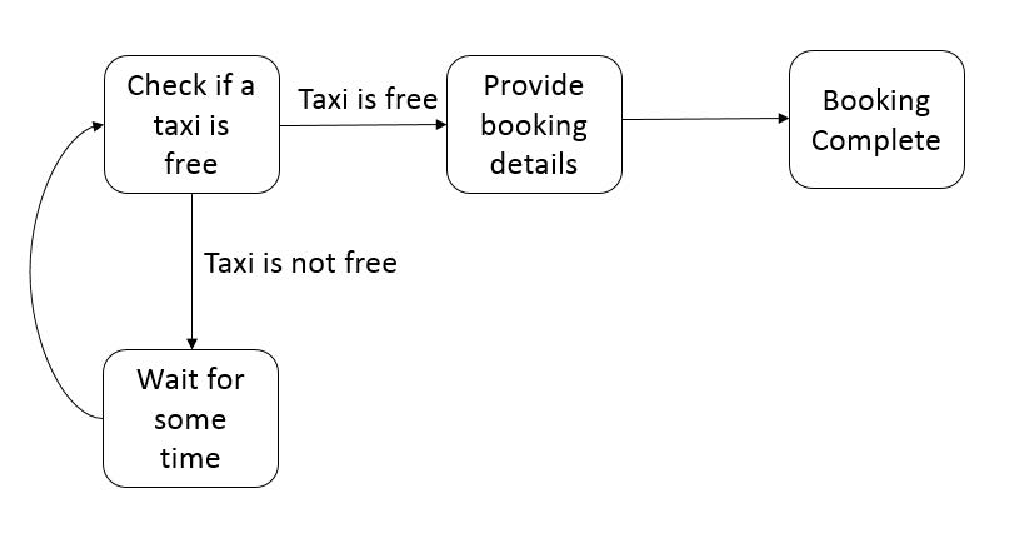
\includegraphics[scale = 0.5]{CPN_abstract_taxi_example.pdf}
	\caption{An abstract model for booking a taxi}
	\label{fig:CPN_abstract_taxi_example}
\end{figure}
\paragraph{\textnormal{Let us consider an example representing a simple online taxi booking service (see Figure \ref{fig:CPN_abstract_taxi_example}). To book a taxi the customer visits the web page. Upon visit, the booking service automatically generates a session identifier. To proceed with the booking process, the system checks for the available taxi. If the taxi is available, then the customer is asked to provide a phone number, pickup time and pickup address. Once the booking information is provided, the booking is finalised and the confirmation is shown to the user. If instead, no taxi is available, the user has to wait until a taxi is free.}}

\section{Coloured Petri Nets (CPNs) Syntax} \label{sec:CPN_Syntax}

\begin{figure}[!htbp]
	\centering
	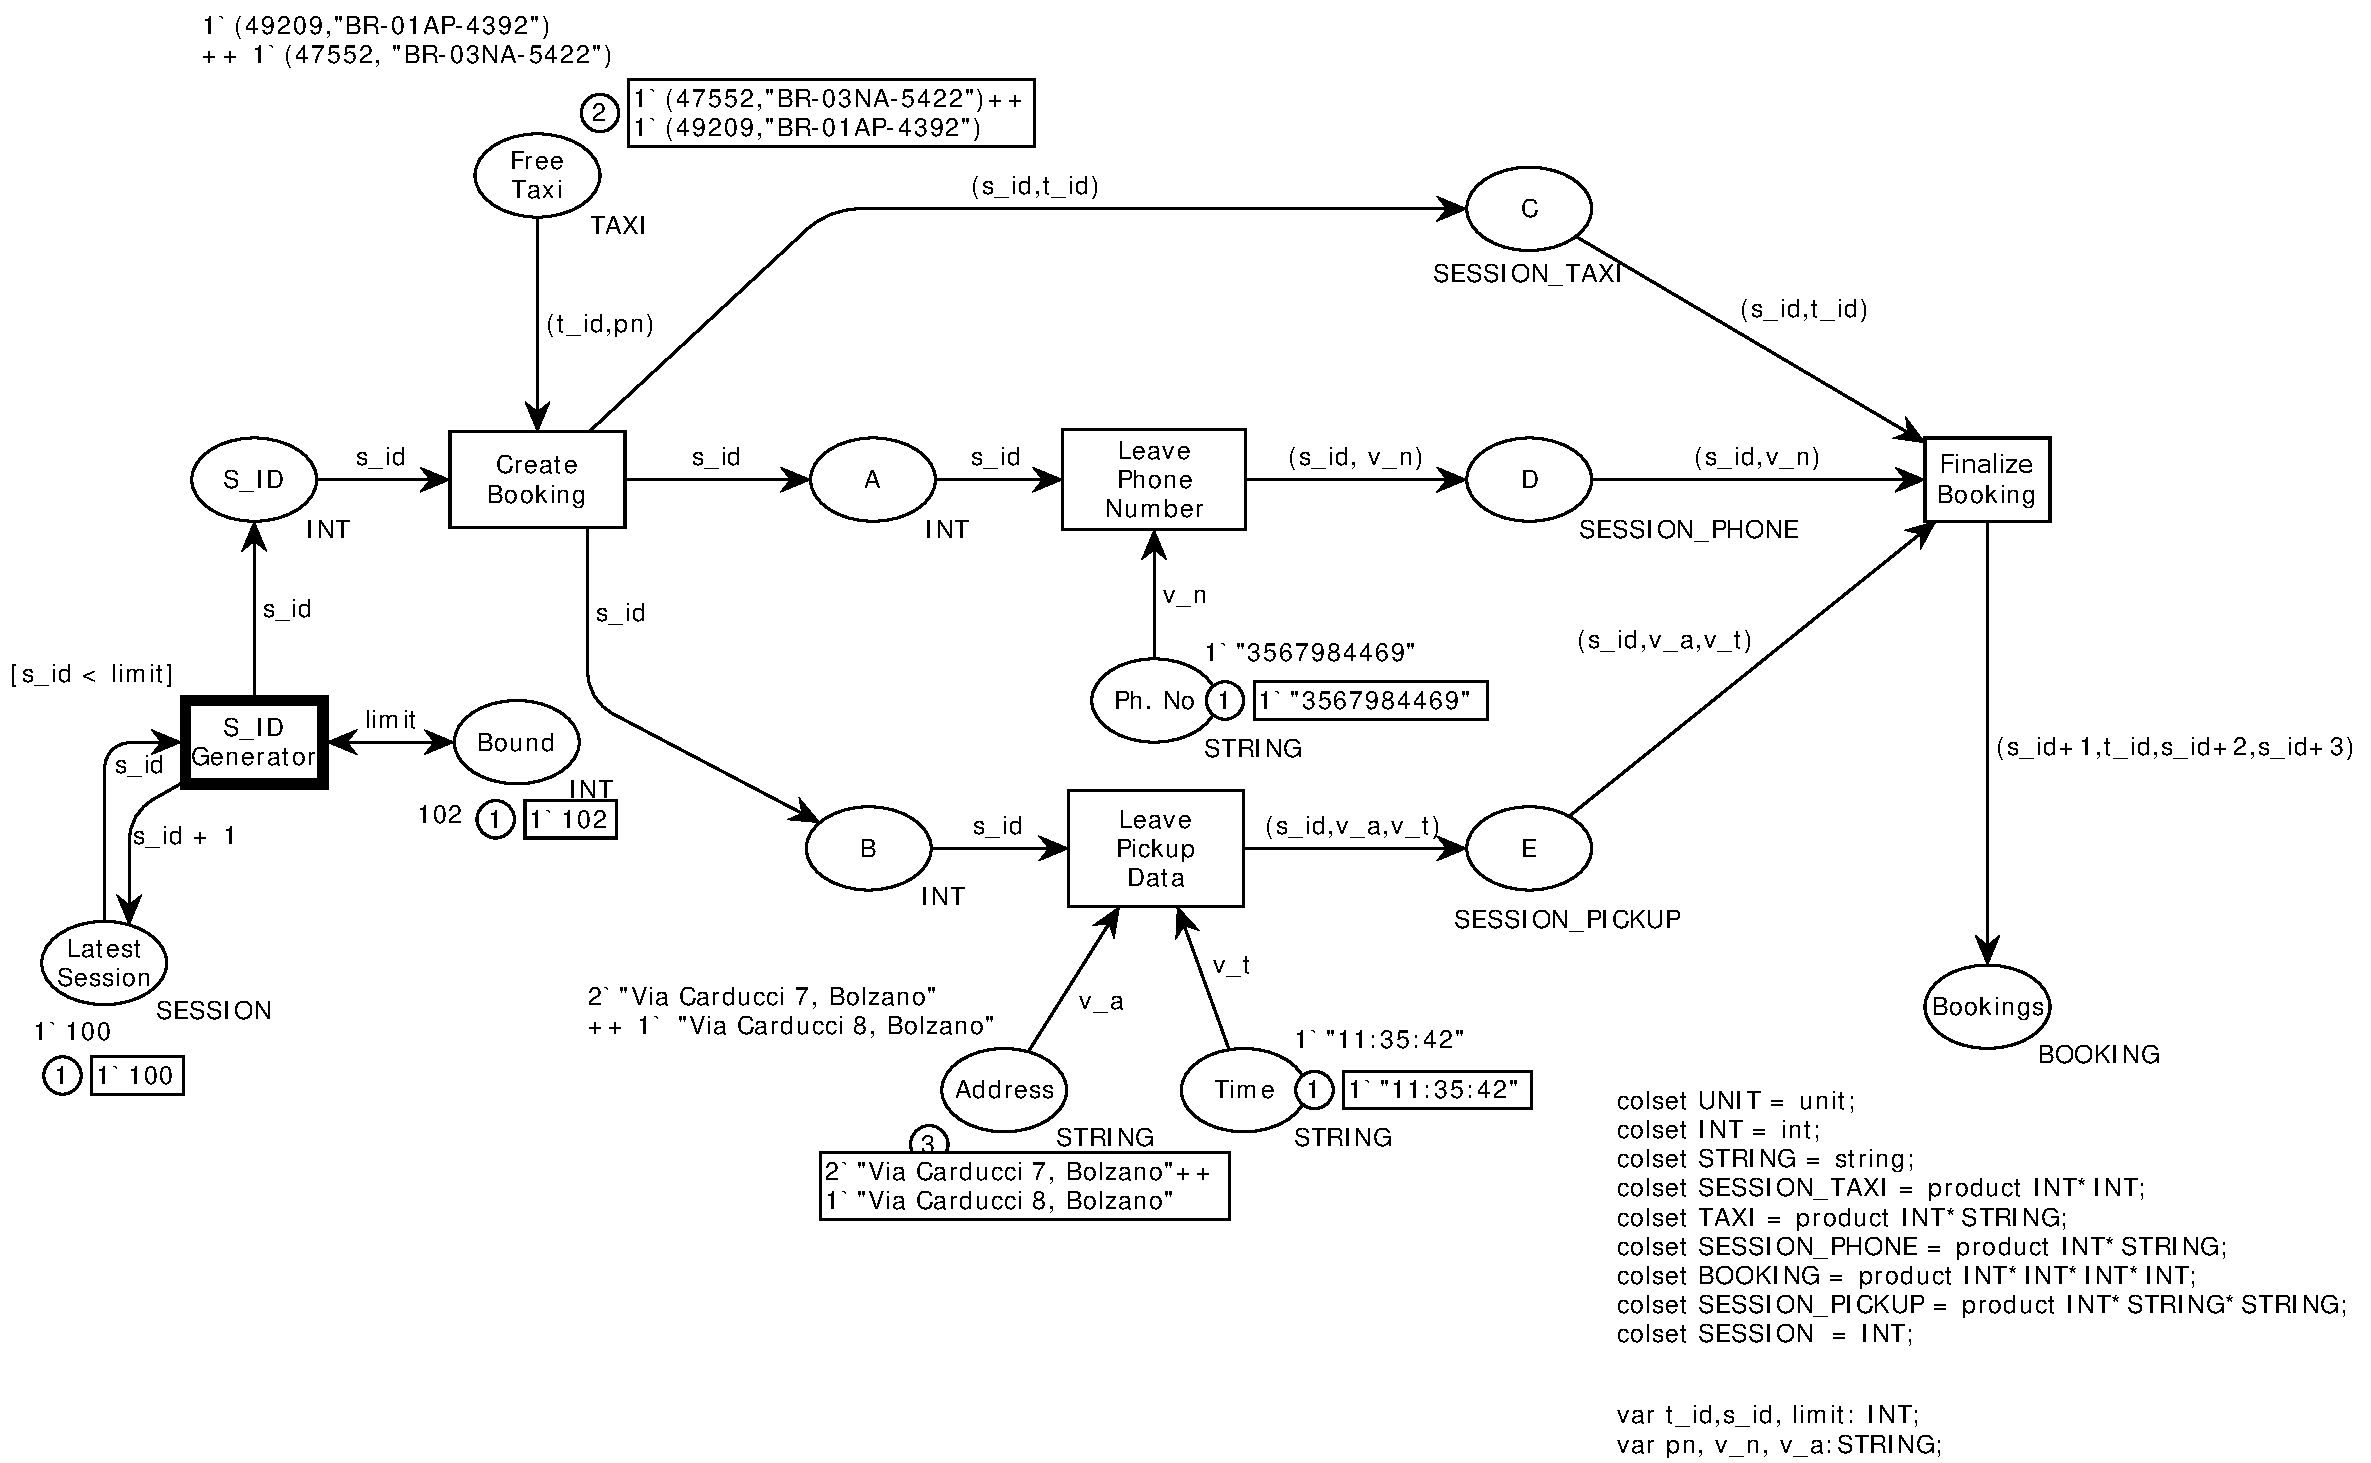
\includegraphics[scale = 0.35]{CPN_Taxi_Booking.pdf}
	\caption{CPN model for taxi booking}
	\label{fig:CPN_Taxi_Booking}
\end{figure}

\subparagraph*{\textnormal{Figure \ref{fig:CPN_Taxi_Booking} shows the CPN model\footnote{This example is modelled in a tool called \bdq{CPN Tools}\cite{CPN_Tools}. CPN Tools uses CPN ML as its programming language.} of the taxi booking example. Here, the places are represented by ellipses and the transitions are represented by rectangles. They are connected to each other by directed arcs. Places represent the state of the system. Each place contains tokens which have data value attached to it. This data value is called \textit{token colour} in CPN. Transitions represent events which can occur in the system. From the classical theory of Petri nets\cite{DBLP:books/daglib/Reisig2013} we know that Petri nets are directed bipartite graph and the bi-partition is between places and transitions, which means that places cannot be connected to places and transitions cannot be connected to transitions.}}

\subparagraph*{\textnormal{A session identifier is generated (at place $\mathit{Latest\ Session}$) incrementally with the starting value as 100. Only 2 session ids can be generated as the guard\footnote{A guard is a boolean expression attached to a transition. In order to make enable a transition, the corresponding guard must evaluate to $\mathit{True}$.} on the $\mathit{S\_ID}$ does not allow to have a session ID greater than the limit which is 102. The transition $\mathit{S\_ID\ Generator}$ is connected to the place $\mathit{Bound}$ with a double headed arc \footnote{It is counted as 2 arcs here, one connecting the place and the transition and the other connecting the same transition and place.}. It does not affect the content of the place. The process proceeds with checking the available taxi and providing the pickup details. $\mathit{Finalize\ Booking}$ transition is called and the confirmed booking is displayed at the place $\mathit{Booking}$. Each booking has a booking id, taxi id, phone id and pickup id. For simplicity and reduced the size of our CPN model, we abstract booking id, taxi id, phone id and pickup id in terms of $\mathit{s\_id}$. We represent them as:
\begin{equation*}
\begin{aligned}
booking\ id = & s\_id + 1\\
phone\ id = & s\_id + 2\\
pickup\ id = & s\_id + 3\\
\end{aligned}
\end{equation*}}}

\subparagraph*{\textnormal{The set of places, transitions, and arcs are denoted by $\mathit{P}$, $\mathit{T}$,and $\mathit{A}$ respectively. In Figure \ref{fig:CPN_Taxi_Booking}, there are 13 places, 5 transitions and 21 directed arcs. The set of places, transitions and arcs are :
\begin{equation*}
\begin{aligned}
P =\ & \{ S\_ID, Free\ Taxi, Address, Time, \ldots \}\footnotemark \\
T =\ &\{ Create\ Booking, Leave\ Phone\ Number, \ldots \} \\
A =\ & \{ (S\_ID, Create\ Booking), (Free\ Taxi, Create Booking),\ldots\}
\end{aligned}
\footnotetext{here in the set notation, \ldots means similarly there are other elements in the set, it should not be confused with an infinite set. The sets are finite.}
\end{equation*}}}

\subparagraph*{\textnormal{In Figure \ref{fig:CPN_Taxi_Booking}, the place $\mathit{Free\ Taxi}$ contains taxis which are not occupied, $\mathit{Bookings}$ contains all the bookings done so far. $\mathit{A}$, $\mathit{B}$, $\mathit{C}$, $\mathit{D}$, $\mathit{E}$ are intermediate places. Places $\mathit{Ph. No}$, $\mathit{Address}$ and $\mathit{Time}$ contain customer's phone number, pickup address and pickup time respectively. For a particular phone number, we have one phone ID which is contained in the place $\mathit{Phone\ ID}$. Similarly, for a booking we have booking id at the place $\mathit{Booking\ ID}$ and for the pickup data, we have a pickup id at place $\mathit{Pickup\ ID}$. The place $\mathit{S\_ID}$ corresponds to session id of a customer. A token is a pair of place and colour-set.}}

\subparagraph*{\textnormal{Each place has a data type attached to it, which is called \textbf{colour-set} of the place. In Figure \ref{fig:CPN_Taxi_Booking}, the colour-set of each place is defined at the bottom right of the place. For example, place $\mathit{S\_ID}$ has the colour-set INT, place $\mathit{Free\ Taxi}$ has the colour-set TAXI. The list of all the colour-set used is provided in Figure \ref{fig:CPN_Taxi_Booking} (in the bottom right corner). In CPN-ML\footnote{CPN Tools uses CPN-ML as its programming language. CPN-ML is an extension of standard ML. Standard ML is a functional programming language, in the sense that the full power of mathematical functions is present. A detailed description of SML is provided in \cite{milner1997definition}. In order to get acquainted with ML programming language in brief and how it used as a programming language with CPN, one can read \cite{Jensen_CPN_Book_ML}.}, the colour-set is written by prefixing the keyword \bdq{COLSET}. The colour-sets STRING and INT are defined as the primitive data type \bdq{string} and \bdq{int} respectively. The colour-set TAXI contains pair (INT, STRING), where the first element represents the taxi id and the second element represents the corresponding plate number.  Similarly, other colour-sets are defined. In general, a colour-set can be cartesian product of different data types.}}

\subparagraph*{\textnormal{We can also restrict the values that a particular colour-set can take. This makes the domain of the colour-set finite\footnote{More information on making finite colour-set is given in \cite{CPN_Tools_ColourSet}}. This is achieved by using the \bdq{with} clause while declaring the colour-set. One such code is provided below. In this code, when we declare the colour-set \bsq{SESSION} we put a limit on the colour-set stating that the value of the integer cannot be less than 100 or greater than 102. Hence by limiting the domain of the colour-set \bsq{SESSION} in the interval $\mathit{\left[100,102\right]}$, we restrict the model to generate a maximum of 2 session ids.}}

\begin{verbatim}
COLSET SESSION = int with 100..102;
\end{verbatim}

\subparagraph*{\textnormal{A \textit{marking} represents the state of the CPN model which is determined by the number of tokens and the token colours on individual places. The marking of a place is determined by the tokens on the specific place. We use the multiset $\mathit{m_{Address}}$ and $\mathit{m_{Free Taxi}}$ to denote the multiset over the colour-set STRING and TAXI respectively corresponding to the markings of the places $\mathit{Address}$ and $\mathit{Free\ Taxi}$ in Figure \ref{fig:CPN_Taxi_Booking}:
\begin{equation*}
\begin{aligned}
&m_{Address} = {2}^{\backprime}\textnormal{"Via Carducci 7, Bolzano"} +\!\!+\ {1}^{\backprime}\textnormal{"Via Carducci 8, Bolzano"}\\
&m_{Free Taxi} = {1}^{\backprime}\textnormal{(49209,\bdsq{(BR-01AP-4392)}} +\!\!+\ {1}^{\backprime}\textnormal{(47552, \bdsq{BR-03NA-5422})}
\end{aligned}
\end{equation*}
This indicates that the place \textit{Address} has the marking which contains 2 tokens of data value \bdsq{Via Carducci 7, Bolzano} and 1 token of data value \bdsq{Via Carducci 8, Bolzano}. The reason for these data values are written in double quotes is because they are of type string. If the number of tokens is 1 then we can omit the number and the ${}^{\backprime}$ operator, and simply write the data value. e.g. ${1}^{\backprime}$\bdsq{Via Carducci 8, Bolzano} can be simply written as \bdsq{Via Carducci 8, Bolzano}. The multiset $m_{Address}$ can be defined as:
\begin{equation*}
m_{Address}(s) = \begin{cases}
2 & \textit{if s = \textnormal{\bdsq{Via Carducci 7, Bolzano}}} \\ 
1 & \textit{if s = \textnormal{\bdsq{Via Carducci 8, Bolzano}}} \\ 
0 & \textit{otherwise}
\end{cases}
\end{equation*}
Similarly, for the place $\mathit{Free\ Taxi}$, one could write it as:
\begin{equation*}
m_{Free Taxi}(s) = \begin{cases}
1 & \textit{if s = \textnormal{(49209,\bdsq{BR-01AP-4392})}} \\ 
1 & \textit{if s = \textnormal{(47552,\bdsq{BR-03NA-5422})}} \\ 
0 & \textit{otherwise} 
\end{cases}
\end{equation*}}}
\begin{comment}
Where the ${}^{\backprime}$ is the infix operator, the number preceding the symbol ${}^{\backprime}$ signifies the number of tokens while the tuple succeeding the symbol represents the data value.	content...
\end{comment}

\subparagraph*{\textnormal{Let us now formally define elements that constitute \textbf{net inscriptions}, i.e., arc expressions, guards and colour-sets. Arc expressions are the expressions written on the arcs. We denote by $\mathit{EXPR}$ the set of expressions provided by the inscription language. Here, the inscription language is a general term for a backend language used to specify colour-sets and operations over them. However, in our case, we rely on a specific language, i.e., CPN ML provided by CPNTools. Given an expression $\mathit{e \in EXPR}$, the \textbf{\textit{type}} of $\mathit{e}$, represented by $\mathit{Type[e]}$, specifies the colour of values obtained by evaluating $\mathit{e}$. The set of \textbf{\textit{free variables}} in an expression $\mathit{e}$ is denoted by $\mathit{Var[e]}$, and the type of a variable $\mathit{v}$ is denoted by $\mathit{Type[v]}$. $\mathit{V}$ denotes the set of variables. Note that a free variable is a variable which is not bound in the local environment of the expression.
In Figure \ref{fig:CPN_Taxi_Booking}, for the arc expressions we have the following free variables:
\begin{equation*}
\mathit{Var[e]} = \begin{cases}
\mathit{\{s\_id\}} & \textit{if e = s\_id}\\ 
\mathit{\{t\_id, pn\}} & \textit{if e = \textnormal{(}t\_id, pn\textnormal{)}} \\ 
\mathit{\{s\_id, t\_id\}} & \textit{if e = \textnormal{(}s\_id, t\_id\textnormal{)}} \\ 
\mathit{\{v\_n\}} & \textit{if e = \textnormal{(}v\_n\textnormal{)}}\\ 
\ldots
\end{cases}
\end{equation*}}}
\subparagraph*{\textnormal{$\mathit{\Sigma}$ denotes the set of \textbf{\textit{colour-sets}} defined for the CPN model. Given a set of variables $\mathit{V}$, for all $\mathit{v \in V : Type[v] \in \Sigma}$. For $\mathit{V' \subseteq V}$, the set of expressions $\mathit{e \in EXPR}$ such that $\mathit{Var[e] \subseteq V'}$ is denoted $\mathit{EXPR_{V'}}$. For the CPN model in Figure \ref{fig:CPN_Taxi_Booking}, the colour-sets are defined as:
\begin{equation*}
\begin{aligned}
\mathit{\Sigma = \{ INT, STRING, TAXI, SESSION\_TAXI, \ldots \}}
\end{aligned}
\end{equation*}
We define the set of free variables in our CPN model:
\begin{equation*}
\begin{aligned}
\mathit{V = \{s\_id : INT, t\_id : INT, v\_a : STRING, v\_t : STRING, \ldots\}}
\end{aligned}
\end{equation*}}}

\subparagraph*{\textnormal{The \textbf{\textit{colour-set function}} is a function, $\mathit{C : P \rightarrow \Sigma}$, which maps every place to its corresponding colour-set. The colour-set function for the CPN model in Figure \ref{fig:CPN_Taxi_Booking} is:}}

\begin{equation*}
C(p) = \begin{cases}
\mathit{INT} & \textit{if p $\in$ \textnormal{\{}S\_ID, A, B, Bound\textnormal{\}}}\\
\mathit{STRING} & \textit{if p $\in$ \textnormal{\{}Ph. No, Address, Time\textnormal{\}}}\\
\mathit{TAXI} & \textit{if p = Free Taxi}\\
\mathit{SESSION\_TAXI} & \textit{if p = C}\\
\mathit{SESSION\_PHONE} & \textit{if p = D}\\
\mathit{SESSION\_PICKUP} & \textit{if p = E}\\
\mathit{BOOKING} & \textit{if p = Bookings} \\
\mathit{SESSION} & \textit{if p = Latest Session}
\end{cases}
\end{equation*}
\paragraph*{\textnormal{\textit{Guard} is a boolean expression attached to the transitions. For a transition be enabled it is a necessary condition that the guard of the transition should evaluate to $\mathit{True}$. A function $\mathit{G : T \rightarrow EXPR_{V}}$ is called a \textbf{\textit{guard function}} and assigns every transition $\mathit{t \in T}$ a boolean expression, i.e., $\mathit{Type[G(t)] = Bool}$. The set of free variables occurring in a guard should be a subset of $\mathit{V}$, hence, $\mathit{G(t) \in EXPR_{V}}$. The CPN model, in Figure \ref{fig:CPN_Taxi_Booking}, has guard function defined as:
}}

\begin{equation*}
G(t) = \begin{cases}
\mathit{s\_id < limit} & $\textit{if t = S\_ID Generator}$\\
\mathit{True} & $\textit{otherwise}$
\end{cases}
\end{equation*}

\subparagraph*{\textnormal{A function $E : A \rightarrow EXPR_{V}$ is called \textbf{\textit{arc expression function}} which assigns every $a \in A$ an expression $E(a)$. Similar to the guards of the transition, the free variables occurring in $E(a)$ has to be a subset of $V$, hence, $E(a) \in EXPR_{V}$. For an arc $(p,t) \in A$, connecting a place $p \in P$ and a transition $t \in T$, it is required that the type of the arc expression is the multiset type over the colour-set $C(p)$ of the place $p$, i.e., $Type[E(p, t)] = C(p)_{MS}$. This is for the directed arc from a place to a transition. Similarly it can be applied to a directed arc from a transition to a place. For an arc $(t,p) \in A$ it is required that $Type[E(t, p)] = C(p)_{MS}$. For the model in Figure \ref{fig:CPN_Taxi_Booking}, the arc expression function is defined as:}}
\begin{equation*}
E(a) = \begin{cases}
{1}^{\backprime}(s\_id) & \textit{if a $\in$ \textnormal{\{(}S\_ID, Create Booking\textnormal{)},}\\
& \textit{\textnormal{(}Create Booking, A\textnormal{)},\textnormal{(}Create Booking, B\textnormal{)},}\\
& \textit{\textnormal{(}A, Leave Phone Number\textnormal{)},}\\ 
& \textit{\textnormal{(}B, Leave Pickup Data\textnormal{)\}}}\\
{1}^{\backprime}(s\_id,t\_id) & \textit{if a $\in$ \textnormal{\{(}Create Booking, C\textnormal{)},}\\ 
& \textit{\textnormal{(}E, Finalize Booking\textnormal{)\}}}\\
{1}^{\backprime}(v\_n) & \textit{if a = \textnormal{(}Ph. No, Leave Phone Number\textnormal{)}}\\
\ldots
\end{cases}
\end{equation*}

\subparagraph*{\textnormal{The initialization function gives initial marking to all places in the model. The \textbf{\textit{initialization function}} $\mathit{I : P \rightarrow EXPR_{0}}$ assigns to each place $\mathit{p}$ an initialization expression $\mathit{I(p)}$ which is required to evaluate to a multiset over the colour-set of the place $\mathit{p}$, i.e., $\mathit{Type[I(p)] = C(p)_{MS}}$. The initialization expression must be a closed expression, i.e., it cannot have any free variables, hence $\mathit{I(p) \in EXPR_{\emptyset}}$. A possible initialization function for the model in Figure \ref{fig:CPN_Taxi_Booking} is given by:
\begin{equation*}
I(p) = \begin{cases}
\textnormal{${1}^{\backprime}$(49209,\bdsq{BR-01AP-4392})} +\!\!+  & \textit{if p = Free Taxi}\\
\textnormal{${1}^{\backprime}$(47552,\bdsq{BR-03NA-5422})} & \\
\textnormal{${2}^{\backprime}$\bdsq{Via Carducci 7, Bolzano}} +\!\!+ & \textit{if p = Address}\\ 
\textnormal{${1}^{\backprime}$\bdsq{Via Carducci 8, Bolzano}} & \\
\textnormal{${1}^{\backprime}$\bdsq{11:35:42}} & \textit{if p = Time}\\
\textnormal{${1}^{\backprime}$\bdsq{3567984469}} & \textit{if p = Ph. No}\\
\textnormal{${1}^{\backprime}$100} & \textit{if p = Latest Session}\\
\textnormal{${1}^{\backprime}$102} & \textit{if p = Bound}\\
\emptyset_{MS} & \textit{otherwise}
\end{cases}
\end{equation*}}}

\subparagraph*{\textnormal{With the explanation of the above functions, we  define non-hierarchical coloured petri nets.}}

\begin{defs}
	\label{defs:CPN_NonHeir}
	A non-hierarchical Coloured Petri Net is a tuple $\mathit{CPN} = \mathit{(P,T,A,\Sigma,V,C,G,E,I)}$, where:
	\begin{itemize}
		\item $\mathit{P}$ is a finite set of places.
		\item $\mathit{T}$ is a finite set of transitions $\mathit{T}$ such that $\mathit{P \cap T = \emptyset}$.
		\item $\mathit{A \subseteq (P \times T) \cup (T \times P)}$ is a set of directed arcs.
		\item $\mathit{\Sigma}$ is a finite set of non-empty colour-sets.
		\item $\mathit{V}$ is a finite set of typed variables such that $\mathit{Type[v] \in \Sigma}$ for all variables $\mathit{v \in V}$.
		\item $\mathit{C : P \rightarrow \Sigma}$ is a colour-set function that assigns a colour-set to each place.
		\item $\mathit{G : T \rightarrow EXPR_{V}}$ is a guard function that assigns a guard to each transition $\mathit{t}$ such that $\mathit{Type[G(t)] = Bool}$.
		\item $\mathit{E : A \rightarrow EXPR_{V}}$ is an arc expression function that assigns an arc expression to each arc $\mathit{a}$ such that $\mathit{Type[E(a)] = C(p)_{MS}}$, where $\mathit{p}$ is the place connected to the arc $\mathit{a}$.
		\item $\mathit{I : P \rightarrow EXPR_{\emptyset}}$ is an initialization function that assigns an initialization expression to each place $\mathit{p}$ such that $\mathit{Type[I(p)] =C(p)_{MS}}$.
	\end{itemize}
\end{defs}

\section{Colored Petri Nets (CPNs) Semantics} \label{sec:CPN_Semantics}
\paragraph{\textnormal{In this section, we discuss about markings and binding elements. Later, we look at a step, enabling and occurrence of steps and when a step occurs how it effects the marking of the net. We also discuss the conditions when the transition is enabled. In the end, we discuss reachable markings and state spaces.}}
\subsection*{Enabling and Occurrence of Steps}

\begin{comment}
\paragraph{\textnormal{In this section, we discuss about markings and binding elements. Later, we look at a step, enabling and occurrence of steps and when a step occurs how it effects the marking of the net. We also discuss the conditions when the transition is enabled. In the end, we discuss reachable markings and state spaces.}}
\end{comment}

\subparagraph{\textnormal{In a given marking, the enabling rule specifies when a step (consisting of a multiset of binding elements) becomes enabled, whereas the firing/occurrence rule specifies how the markings change when the enabled step occurs.}}

\begin{figure}[!htbp]
	\centering
	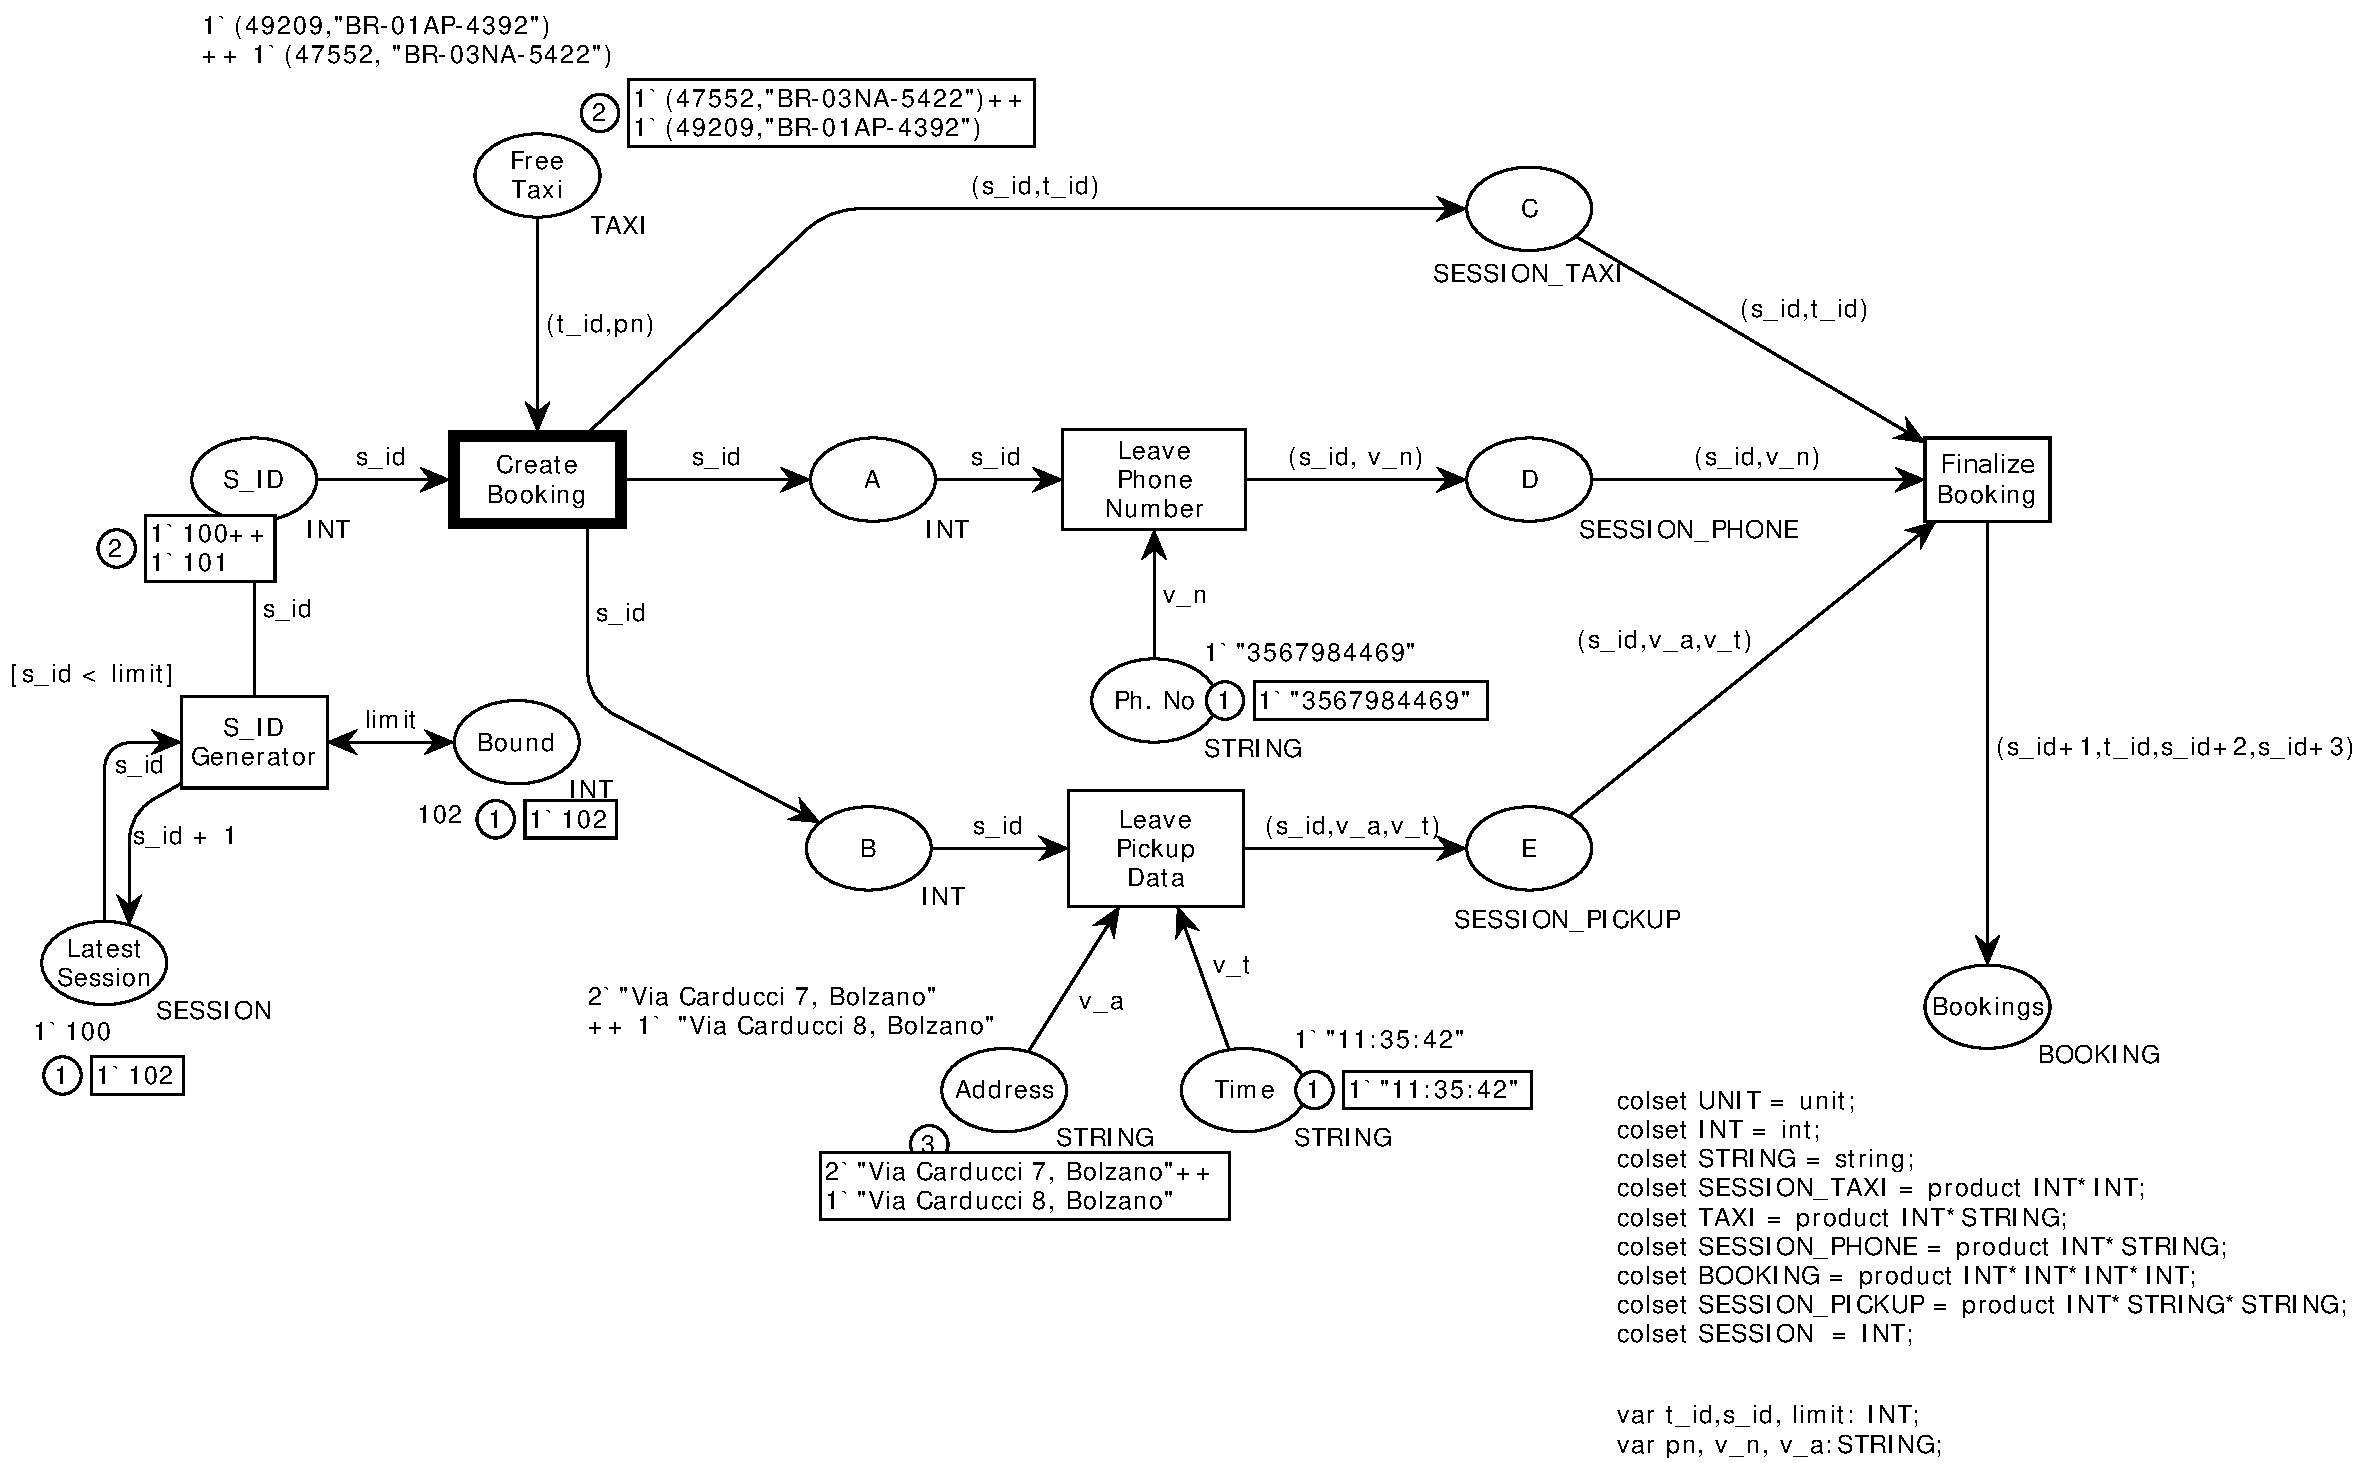
\includegraphics[scale = 0.35]{CPN_Taxi_Booking_initial_step.pdf}
	\caption{CPN model for taxi booking}
	\label{fig:CPN_Taxi_Booking_initial_step}
\end{figure}

\subparagraph*{\textnormal{A \textbf{\textit{marking}} $\mathit{M}$ is a function that maps each place $\mathit{p}$ into a multiset of values $\mathit{M(p)}$ representing the marking of $\mathit{p}$. The individual elements in the multiset $\mathit{M(p)}$ are called \textbf{\textit{tokens}}. The multiset of tokens present on a place $\mathit{p}$ in a marking $\mathit{M}$ is required to match the type of the place, i.e., $\mathit{M(p) \in C(p)_{MS}}$. For example, the marking of the places for the CPN model presented in Figure \ref{fig:CPN_Taxi_Booking_initial_step} is given by\footnote{The markings in the model are represented by rectangles beside each place.}:}}

\begin{equation*}
M(p) = \begin{cases}
{1}^{\backprime}100 +\!\!+ {1}^{\backprime}101 & \textit{if p = S\_ID}\\
\textnormal{${1}^{\backprime}$(49209,\bdsq{BR-01AP-4392})} +\!\!+  & \textit{if p = Free Taxi}\\
\textnormal{${1}^{\backprime}$(47552,\bdsq{BR-03NA-5422})} & \\
\textnormal{${2}^{\backprime}$\bdsq{Via Carducci 7, Bolzano}} +\!\!+ & \textit{if p = Address}\\ 
\textnormal{${1}^{\backprime}$\bdsq{Via Carducci 8, Bolzano}} & \\
\textnormal{${1}^{\backprime}$\bdsq{11:35:42}} & \textit{if p = Time}\\
\textnormal{${1}^{\backprime}$\bdsq{3567984469}} & \textit{if p = Ph. No}\\
\textnormal{${1}^{\backprime}$102} & \textit{if p = Latest Session}\\
\textnormal{${1}^{\backprime}$102} & \textit{if p = Bound}\\
\emptyset_{MS} & \textit{otherwise}
\end{cases}
\end{equation*}

\subparagraph*{\textnormal{$\mathit{Var(t)}$ denotes \textbf{\textit{variables of a transition}} $\mathit{t}$, which consists of free variables appearing either in any of the arc expression connecting the transition or in the guard of the transition. The variables for the transitions for the model in the Figure \ref{fig:CPN_Taxi_Booking_initial_step} are:}}
\begin{equation*}
Var(t) = \begin{cases}
\{s\_id,t\_id,pn\} & \textit{if t = Create Booking}\\
\{s\_id,v\_n\} & \textit{if t = Leave Phone Number}\\
\{s\_id,v\_a,v\_t\} & \textit{if t = Leave Pickup Data}\\
\{s\_id,t\_id,v\_n,v\_a,v\_t\} & \textit{if t = Finalize Booking}\\
\{s\_id,limit\} & \textit{if t = S\_ID Generator} 
\end{cases}
\end{equation*}

\subparagraph*{\textnormal{The \textbf{\textit{initial marking}}, denoted by $\mathit{M_{0}}$, is obtained by evaluating the initialization expression. The initialization expression does not contain any free variables and its evaluation is with the empty binding (denoted by $\mathit{\langle \rangle}$), i.e., $\mathit{M_{0}(p) = I(p)\langle \rangle,}$ for each $\mathit{p \in P}$. The initial marking for this example (Figure \ref{fig:CPN_Taxi_Booking}) is given by:}}

\begin{equation*}
M_{0}(p) = \begin{cases}
\textnormal{${1}^{\backprime}$(49209,\bdsq{BR-01AP-4392})} +\!\!+  & \textit{if p = Free Taxi}\\
\textnormal{${1}^{\backprime}$(47552,\bdsq{BR-03NA-5422})} & \\
\textnormal{${2}^{\backprime}$\bdsq{Via Carducci 7, Bolzano}} +\!\!+ & \textit{if p = Address}\\ 
\textnormal{${1}^{\backprime}$\bdsq{Via Carducci 8, Bolzano}} & \\
\textnormal{${1}^{\backprime}$\bdsq{11:35:42}} & \textit{if p = Time}\\
\textnormal{${1}^{\backprime}$\bdsq{3567984469}} & \textit{if p = Ph. No}\\
\textnormal{${1}^{\backprime}$100} & \textit{if p = Latest Session}\\
\textnormal{${1}^{\backprime}$102} & \textit{if p = Bound}\\
\emptyset_{MS} & \textit{otherwise}
\end{cases}
\end{equation*}

\subparagraph*{\textnormal{A \textbf{\textit{binding}} $b$ of a transition $t$ is a function that maps each variable $v$ of the transition $t$ to a value $b(v)$ belonging to the type of the variable $v$, i.e., $b(v) \in Type[v]$. Bindings are written as $\langle var_{1} = val_{1},var_{2} = val_{2}, \ldots ,var_{n} = val_{n} \rangle$, where $var_{1}, var_{2}, \ldots , var_{n}$ are the variables in $Var(t)$ and $val_{i}$ is the value bound to the variable $var_{i}$. A \textbf{\textit{binding element}} is a pair $(t,b)$ consisting of a transition $t$ and a binding $b$ of $t$. A step is a non-empty, finite multiset of binding elements.}}

\subparagraph*{\textnormal{With the above functions at hand, we define few concepts related to CPN.}}

\begin{defs}
	\label{defs:2_7_step_marking}
	For a Coloured Petri Net $\mathit{CPN = (P,T,A,\Sigma,V,C,G,E,I)}$:
	\begin{enumerate}
		\item A \textbf{marking} is a function $\mathit{M}$ that maps each place $\mathit{p \in P}$ into a multiset of tokens
		$\mathit{M(p) \in C(p)_{MS}}$.
		\item The \textbf{initial marking} $\mathit{M_{0}}$ is defined by $\mathit{M_{0}(p) = I(p)}$ for all $\mathit{p \in P}$.
		\item The \textbf{variables of a transition} $\mathit{t}$ are denoted $\mathit{Var(t) \subseteq V}$ and consist of the free variables appearing in the guard of $\mathit{t}$ and in the arc expressions of arcs connected to $\mathit{t}$.
		\item A \textbf{binding} of a transition $\mathit{t}$ is a function $\mathit{b}$ that maps each variable $\mathit{v \in Var(t)}$ into a value $\mathit{b(v) \in Type[v]}$. The set of all bindings for a transition $\mathit{t}$ is denoted $\mathit{B(t)}$.
		\item A \textbf{binding element} is a pair $\mathit{(t,b)}$ such that $\mathit{t \in T}$ and $\mathit{b \in B(t)}$. The set of all binding elements $\mathit{BE(t)}$ for a transition $\mathit{t}$ is defined by $\mathit{BE(t)} = \mathit{\{(t,b) | b \in B(t)\}}$. The set of all binding elements in a CPN model is denoted $\mathit{BE}$.
		\item A \textbf{step} $\mathit{Y \in BE_{MS}}$ is a non-empty, finite multiset of binding elements.
	\end{enumerate}
\end{defs}

\subparagraph*{\textnormal{As stated earlier, the transitions have guards attached to them and the arcs carry expressions with them (arc expressions). These two determine the enabling and occurrence of a step. For a binding element $\mathit{(t,b)}$ where $\mathit{t}$ is a transition and $\mathit{b}$ is a binding, the guard expression $\mathit{G(t)}$ of the transition is evaluated against the binding $\mathit{b}$ and the result is written as $\mathit{G(t)\langle b \rangle}$. Similarly, the arc expression $\mathit{E(a)}$ (for any arc $\mathit{a}$) is also evaluated against the binding $\mathit{b}$ and the result is written as $\mathit{E(a)\langle b \rangle}$. For an arc $\mathit{a = (p,t)}$, which connects a place $\mathit{p}$ and a transition $\mathit{t}$, the arc expression $\mathit{E(p,t)}$ denotes the arc expression on the input arc from $\mathit{p}$ to $\mathit{t}$. When no such arc exists, we define $\mathit{E(p, t) = \emptyset_{MS}}$. Analogously, $\mathit{E(t, p)}$ denotes the arc expression on the output arc from $\mathit{t}$ to $\mathit{p}$. When no such arc exists, we define $\mathit{E(t, p) = \emptyset_{MS}}$.}}

\subparagraph*{\textnormal{For a binding $\mathit{(t,b)}$ to be enabled in a making $M$ there are two conditions to satisfy:
\begin{itemize}
\item The evaluation of the guard expression - In order for a binding to get enabled, the corresponding guard expression must evaluate to $\mathit{True}$.
\item The number of tokens in the input place - for each place $\mathit{p}$, an arc expression $\mathit{E(p,t)}$ has to be evaluated to the binding $\mathit{b}$ such that $\mathit{E(p,t)\langle b \rangle\ll=M(P)}$. It means that for each place $\mathit{p}$ there should be enough tokens that transition $\mathit{t}$ will remove when occurring with binding $\mathit{b}$.
\end{itemize}
}}

\subparagraph*{\textnormal{Let us look at the two conditions in our taxi booking example. Since we do not have any guards on our model the guard function evaluates to $\mathit{True}$ for all transitions in the model. Let us consider a binding element $\mathit{(Create\ Booking, b_{CB})}$ where
\begin{equation}
\label{eq:binding_1}
b_{CB} = \langle s_{id} = 100, t_{id} = 47552, pn = \textnormal{"BR-03NA-5422"}\rangle
\end{equation}
Alternatively, $b_{CB}$ can also be chosen as:
\begin{equation}
\label{eq:binding_2}
b_{CB} = \langle s_{id} = 101, t_{id} = 49209, pn = \textnormal{"BR-01AP-4392"}\rangle
\end{equation}
One of the important properties of CPN is non-determinism. Here, the values for the binding $\mathit{b_{CB}}$ can be chosen non-deterministically. Here, we will select the binding given in equation \ref{eq:binding_1}. From the input arcs of the $\mathit{Create\ Booking}$ transition, we have
\begin{equation*}
\begin{aligned}
E(S\_ID, Create\ Booking)\langle b_{CB}\rangle =& {1}^{\backprime}100 \ll = {1}^{\backprime}100\ +\!\!+\ {1}^{\backprime}101\\
E(Free\ Taxi, Create\ Booking)\langle b_{CB}\rangle =& {1}^{\backprime}(47552,\textnormal{"BR-03NA-5422"})\\ 
& \ll = {1}^{\backprime}(49209,\textnormal{"BR-01AP-4392"}) +\!\!+\ \\
& {1}^{\backprime}(47552,\textnormal{"BR-03NA-5422"})
\end{aligned}
\end{equation*}}}

\subparagraph*{\textnormal{When an enabled binding $\mathit{(t,b)}$ occurs \footnote{The thick border around the transition (see Figure \ref{fig:CPN_Taxi_Booking_initial_step}) signifies that the transition is enabled.}, the tokens are consumed from the input place and produced at the output place. The amount of tokens consumed or produced depends on the arc inscription attached to the respective arcs. The multiset of tokens removed from the input place $\mathit{p}$, when $\mathit{t}$ occurs in $\mathit{b}$ is given by $\mathit{E(p,t)\langle b \rangle}$, and the multiset of tokens added to an output place $\mathit{p}$ is given by: $\mathit{E(t,p)\langle b \rangle}$, which means that the new marking $\mathit{M'}$ reached when an enabled binding element $\mathit{(t,b)}$ occurs in a marking $\mathit{M}$ is given by:
\begin{equation*}
M'(p) = (M(p) -\!-\ E(p, t)\langle b \rangle) +\!\!+\ E(t, p)\langle b \rangle , \forall p \in P
\end{equation*}}}

\subparagraph*{\textnormal{For our model in Figure \ref{fig:CPN_Taxi_Booking}, let us calculate the new marking $M^{'}$ assuming the binding element (\textit{Create Booking, $b_{CB}$}) occurs.}}
\begin{equation*}
\begin{aligned}
M^{'}(S\_ID) =\ & ({1}^{\backprime}100\ +\!\!+\ {1}^{\backprime}101 -\!- \ {1}^{\backprime}100) +\!\!+\ \emptyset_{MS}\\
=\ & {1}^{\backprime}101 \\
M^{'}(Free\ Taxi) =\ & ({1}^{\backprime}(49209,\textnormal{"BR-01AP-4392"}) +\!\!+\ {1}^{\backprime}(47552,\textnormal{"BR-03NA-5422"})\\  
& -\!-\ {1}^{\backprime}(47552,\textnormal{"BR-03NA-5422"})) +\!\!+\ \emptyset_{MS}\\ 
=\ & {1}^{\backprime}(49209,\textnormal{"BR-01AP-4392"})\\ 
M^{'}(A) =\ &(\emptyset_{MS} -\!-\ \emptyset_{MS}) +\!\!+\ {1}^{\backprime}100 \\
=\ &{1}^{\backprime}100\\
M^{'}(B) =\ &(\emptyset_{MS} -\!-\ \emptyset_{MS}) +\!\!+\ {1}^{\backprime}100 \\
=\ &{1}^{\backprime}100\\
M^{'}(C) =\ &(\emptyset_{MS} -\!-\ \emptyset_{MS}) +\!\!+\ {1}^{\backprime}(100,47552)\\
=\ &{1}^{\backprime}(100,47552)
\end{aligned}
\end{equation*}

\begin{figure}[!htbp]
	\centering
	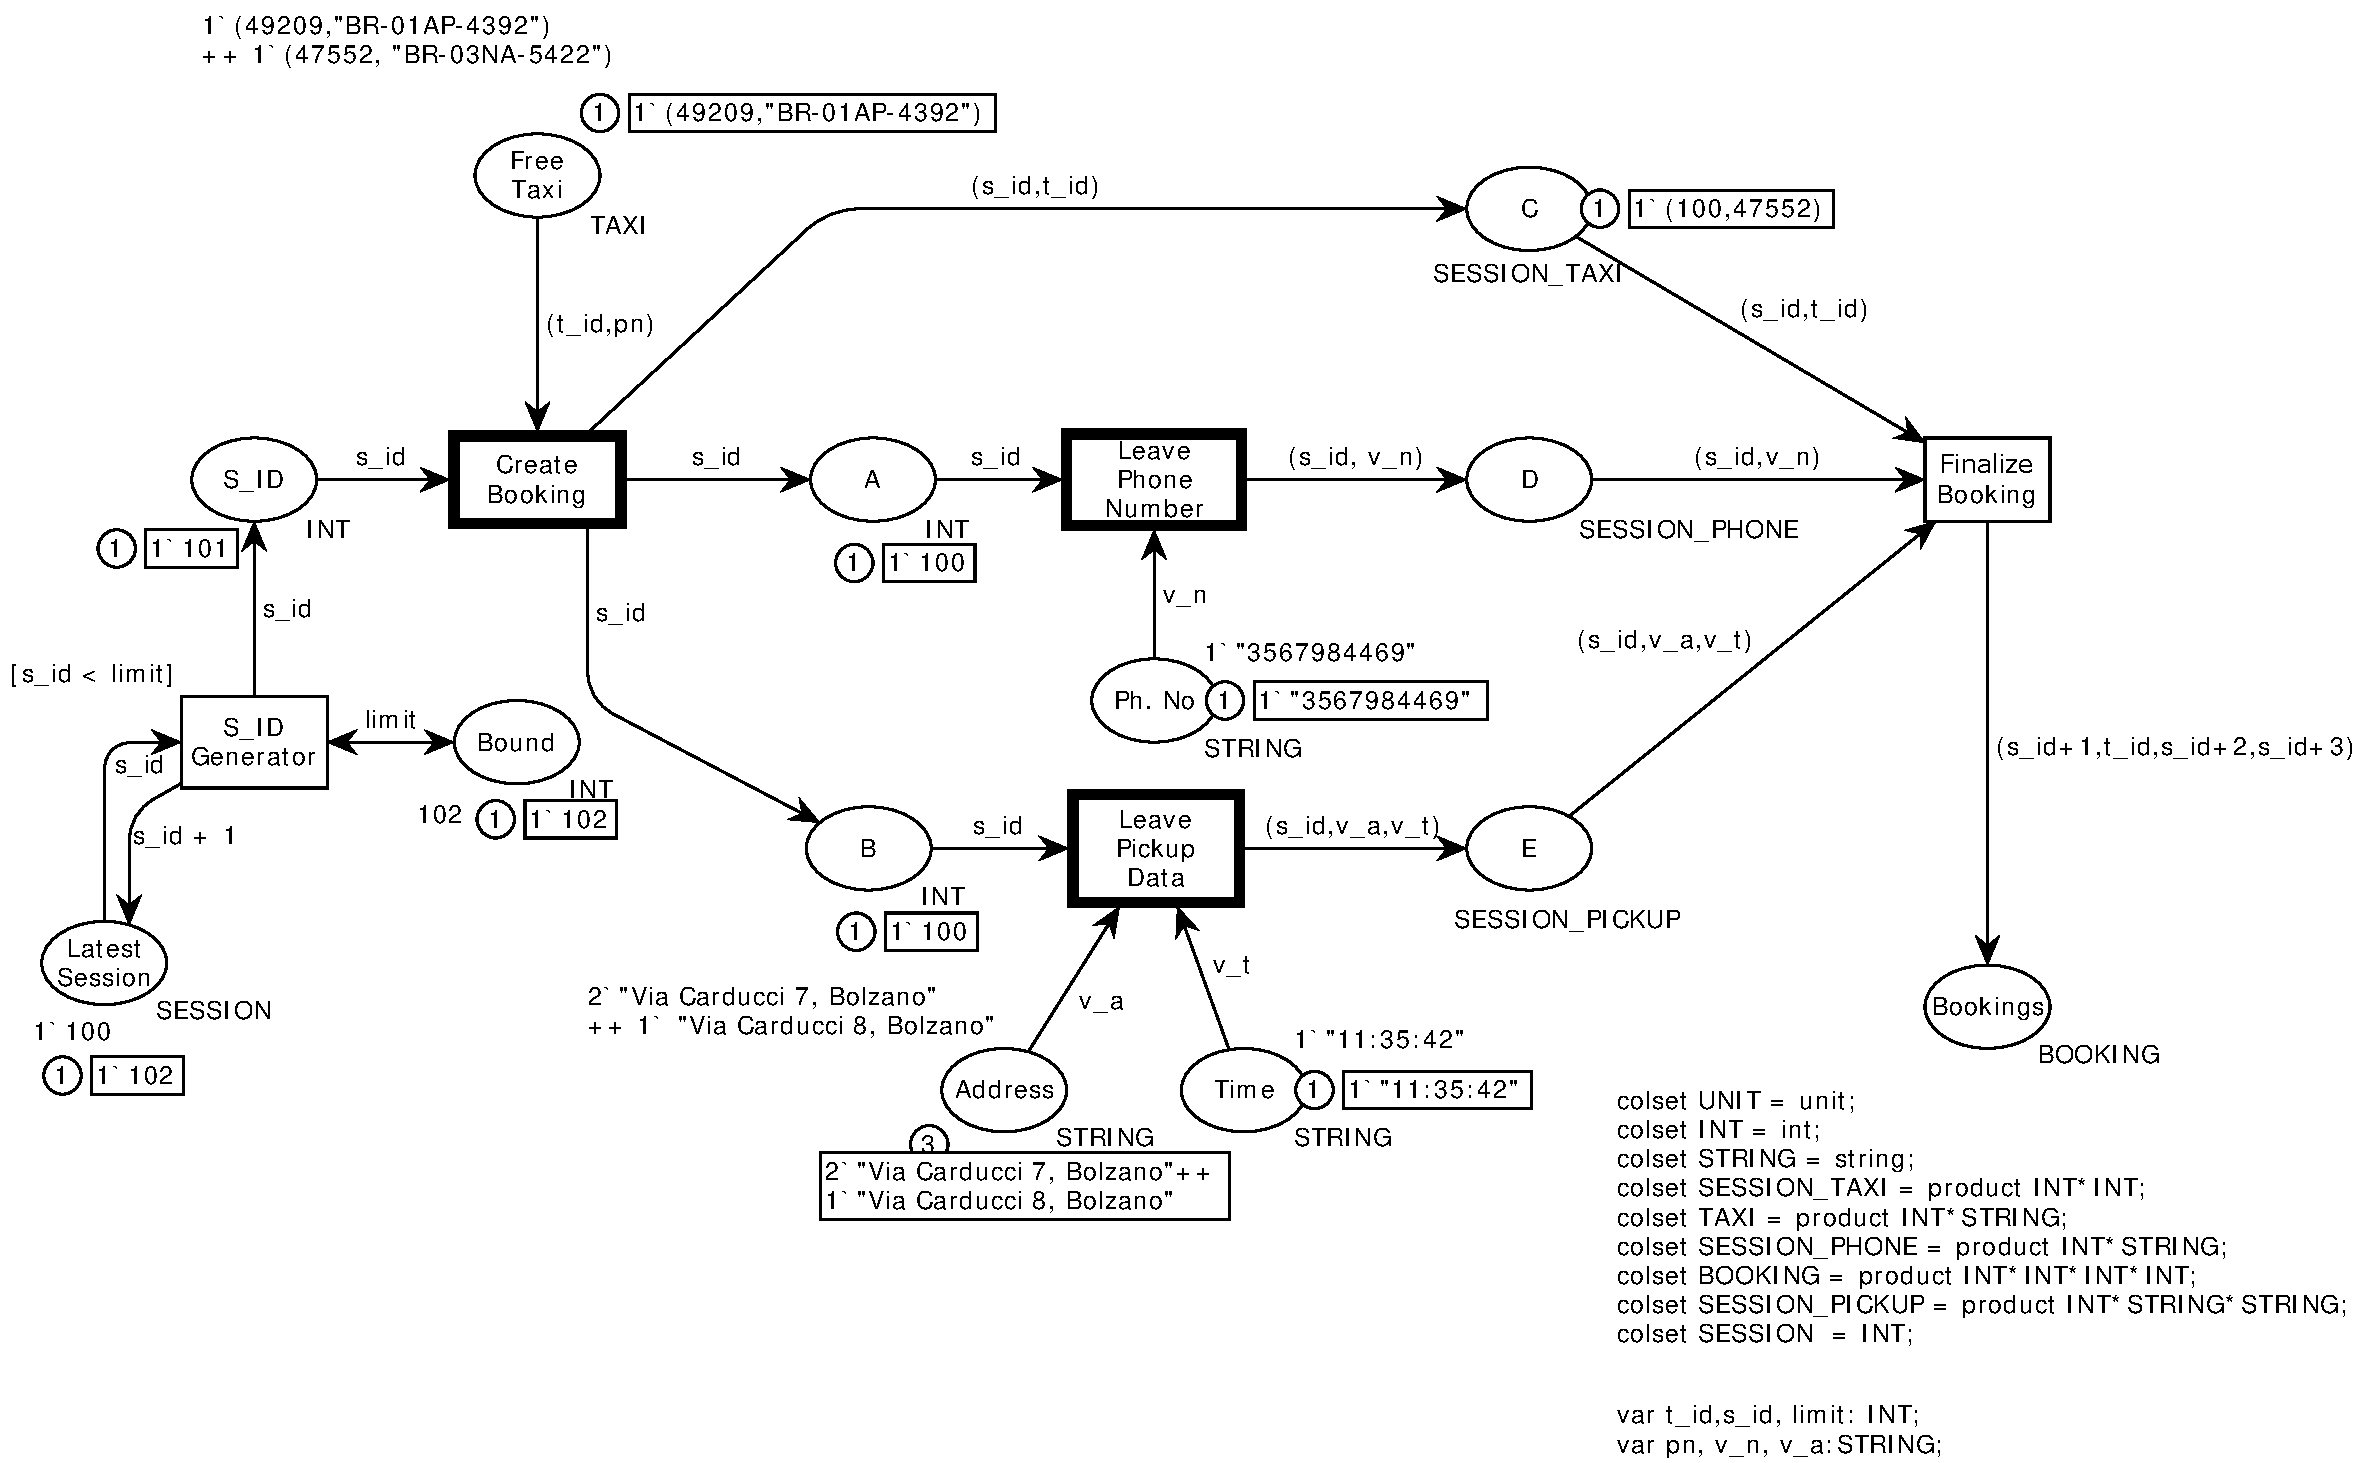
\includegraphics[scale = 0.35]{CPN_Taxi_Booking_one_step.pdf}
	\caption{A state of the CPN model for taxi booking}
	\label{fig:CPN_Taxi_Booking_one_step}
\end{figure}

\subparagraph*{\textnormal{In Figure \ref{fig:CPN_Taxi_Booking_one_step}, there are 3 transitions which are enabled, namely, $\mathit{Create\ Booking}$, $\mathit{Leave\ Phone\ Number}$ and $\mathit{Leave\ Pickup\ Data}$. This is the synchronization property of CPNs where there are multiple transitions enabled and each such transition may fire. The simulation(execution of transitions) is halted when there are no more enabled transitions.}}

\subparagraph*{\textnormal{Now with the explanation of how we can determine enabling and occurrence of steps, let us visit the definition of enabling and occurrence of a binding element in a coloured Petri net.}}
\begin{defs}
	\label{defs:enabling_binding_cpn}
	A binding element $\mathit{(t,b) \in BE}$ is \textbf{enabled} in a marking $\mathit{M}$ if and only
	if the following two properties are satisfied:
	\begin{enumerate}
		\item $\mathit{G(t)\langle b \rangle}$.
		\item $\mathit{\forall p \in P : E(p,t)\langle b \rangle \ll= M(p)}$.
		\item When $\mathit{(t,b)}$ is enabled in $\mathit{M}$, it may \textbf{occur}, leading to the marking $\mathit{M}$ defined by:
		\begin{equation*}
			\forall p \in P : M'(p) = \left(M(p) -\!- E(p,t)\langle b \rangle \right) +\!\!+ E(t, p)\langle b \rangle.
		\end{equation*}
	\end{enumerate}
\end{defs}

\subparagraph*{\textnormal{We have already covered enabling and occurrence of bindings. Now let us consider the enabling and occurrence of steps. In a step $\mathit{Y}$, each binding element (included in the step) should satisfy the guard of the transition $t$. Also, each place $\mathit{p}$ must have the marking $\mathit{M(p)}$ greater than or equal to the sum of the tokens that are removed from $\mathit{p}$.
		\begin{equation*}
		^{++}_{MS} \sum\limits_{(t,b) \in Y} E(p,t)\langle b \rangle \ll= M(p)
		\end{equation*}
		where MS to the lower left of the summation symbol specifies that
		we are adding a multiset of multisets. Each term $E(p, t)\langle b \rangle$ occurs as many times in the sum as $(t,b)$ occurs in $Y$.}}

\subparagraph*{\textnormal{The new marking $\mathit{M'}$ reached when an enabled step $\mathit{Y}$ occurs in a
		marking $\mathit{M}$ is given by:
		\begin{equation*}
			M'(p) = \left(M(p) -\!- ^{++}_{MS} \sum\limits_{(t,b) \in Y} E(p,t)\langle b \rangle \right)\ +\!\!+\ ^{++}_{MS}\sum\limits_{(t,b) \in Y} E(t,p)\langle b \rangle \forall p \in P
\end{equation*}}}

\subparagraph*{\textnormal{The state of the model after firing the transition $\mathit{Create\ Booking}$ with the binding $\mathit{b_{CB}}$ is shown in Figure \ref{fig:CPN_Taxi_Booking_one_step}. In a summarized way let us call the markings at this state of the system as $\mathit{M_{1}}$.
\begin{equation*}
M_{1}(p) = \begin{cases}
\textnormal{${1}^{\backprime}$101} & \textit{if p = S\_ID}\\
\textnormal{${1}^{\backprime}$(49209,\bdsq{BR-01AP-4392})}  & \textit{if p = Free Taxi}\\
\textnormal{${2}^{\backprime}$\bdsq{Via Carducci 7, Bolzano}} +\!\!+ & \textit{if p = Address}\\ 
\textnormal{${1}^{\backprime}$\bdsq{Via Carducci 8, Bolzano}} & \\
\textnormal{${1}^{\backprime}$\bdsq{11:35:42}} & \textit{if p = Time}\\
\textnormal{${1}^{\backprime}$\bdsq{3567984469}} & \textit{if p = Ph. No}\\
\textnormal{${1}^{\backprime}$100} & \textit{if p $\in$ \textnormal{\{}A, B\textnormal{\}}}\\
\textnormal{${1}^{\backprime}$(100,47552)} & \textit{if p = C}\\
\textnormal{${1}^{\backprime}$102} & \textit{if p = Latest Session}\\
\textnormal{${1}^{\backprime}$102} & \textit{if p = Bound}\\
\emptyset_{MS} & \textit{otherwise}
\end{cases}
\end{equation*}
The enabling and occurrence of a step can be defined as below:}}
\begin{defs}
	\label{defs:enabling_steps_cpn}
	A step $\mathit{Y \in BE_{MS}}$ is \textbf{enabled} in a marking $\mathit{M}$ if and only if the following
	two properties are satisfied:
	\begin{enumerate}
		\item $\mathit{\forall (t,b) \in Y : G(t)\langle b \rangle}$.
		\item $\mathit{\forall p \in P :\ ^{++}_{MS} \sum\limits_{(t,b) \in Y} E(p,t)\langle b \rangle \ll= M(p)}$
		\item When $\mathit{Y}$ is enabled in $\mathit{M}$, it may \textbf{occur}, leading to the marking $\mathit{M'}$ defined by:
		\begin{equation*}
			\forall p \in P : M'(p) = \left(M(p) -\!- ^{++}_{MS} \sum\limits_{(t,b) \in Y} E(p,t)\langle b \rangle \right)\ +\!\!+\ ^{++}_{MS}\sum\limits_{(t,b) \in Y} E(t,p)\langle b \rangle
		\end{equation*}
	\end{enumerate}
\end{defs}

\subparagraph*{\textnormal{Now we represent that the marking $\mathit{M_{2}}$ is directly reachable from $\mathit{M_{1}}$ by the step $\mathit{Y}$ by :
		\begin{center}
			$\mathit{M_{1} \xrightarrow{Y} M_{2}}$ or simply by $\mathit{M_{1} \xrightarrow{} M_{2}}$
		\end{center}
}}
\begin{defs}
	\label{defs:finite_occurrence_seq}
	A \textbf{finite occurrence sequence of length} $\mathit{n \geq 0}$ is an alternating sequence
	of markings and steps, written as
	\begin{equation*}
		M_{1} \xrightarrow{Y_{1}} M_{2} \xrightarrow{Y_{2}} M_{3} \ldots M_{n} \xrightarrow{Y_{n}} M_{n+1}
	\end{equation*}
	such that $\mathit{M_{i} \xrightarrow{Y_{i}} M_{i+1}}$ for all $\mathit{1 \leq i \leq n}$. All markings in the sequence are said to
	be \textbf{reachable} from $\mathit{M_{1}}$. This implies that an arbitrary marking $\mathit{M}$ is reachable from
	itself by the trivial occurrence sequence of length 0.\\
	Analogously, an \textbf{infinite occurrence sequence} is a sequence of markings and
	steps
	\begin{equation*}
		M_{1} \xrightarrow{Y_{1}} M_{2} \xrightarrow{Y_{2}} M_{3} \xrightarrow{Y_{3}} \ldots
	\end{equation*}
	such that $\mathit{M_{i} \xrightarrow{Y_{i}} M_{i+1}, \forall i \geq 1}$. The set of markings reachable from a marking $\mathit{M}$ is denoted $\mathit{\mathscr R(M)}$. The set of \textbf{reachable markings} is $\mathit{\mathscr R(M_{0})}$, i.e., the set of markings reachable from the initial marking $\mathit{M_{0}}$.
\end{defs}

\paragraph*{State Spaces}
\subparagraph*{\textnormal{The \textit{state space} of a CPN model is a directed graph $\mathit{SS}$, comprising a set of nodes $\mathit{N_{SS}}$ which corresponds to set of reachable markings $\mathit{\mathscr R(M_{0})}$ and a set of directed arcs represented by $\mathit{A_{SS}}$. An arc $\mathit{a \in A_{SS}}$ connects two nodes $\mathit{M}$ and $\mathit{M^{'}}$ and has a label of binding element $\mathit{(t,b)}$ on it iff $\mathit{(t,b)}$ is enabled in marking $\mathit{M}$ and occurrence of $\mathit{(t,b)}$ leads to the marking $\mathit{M^{'}}$, i.e., $\mathit{M \xrightarrow{(t,b)} M^{'}}$. The state space is finite if the set of reachable markings is finite and the set of enabled bindings in each reachable marking is also finite. The formal definition of the state space for a CPN model is:}}
\begin{defs}
	\label{defs:state_space}
	The \textbf{state space} of a Coloured Petri Net is a directed graph $\mathit{SS =
	(N_{SS},A_{SS})}$ with arc labels from BE, $\mathit{M_{0}}$ is the initial marking and M being an intermediate marking, where:
	\begin{enumerate}
		\item $\mathit{N_{SS} = \mathscr R(M_{0})}$ is the set of \textbf{nodes}.
		\item $\mathit{A_{SS} = \{ (M,(t,b),M^{'}) \in N_{Ss} \times BE \times N_{SS}\ | M \xrightarrow{(t,b)} M^{'} \}} $ is the set of \textbf{arcs}.
	\end{enumerate}
	$SS$ is finite if and only if $\mathit{N_{SS}}$ and $\mathit{A_{SS}}$ are finite.
\end{defs}

\subparagraph*{\textnormal{For the CPN model in Figure \ref{fig:CPN_Taxi_Booking}, there are more than 50 nodes and more than 100 arcs in the state space which makes it difficult to show all the states. For simplicity, we slightly change our model and our new model is shown in Figure \ref{fig:CPN_Taxi_Booking_simple}. In this model, we removed the transition \textit{S\_ID Generator} and fixed the assume that only a single session identifier is generated. Also, for simplicity, some tokens are removed from the place \bsq{Address}. While drawing the state space, we label the nodes with the marking of the model and arcs with the fired transition and the corresponding binding element. The state space of this CPN model is shown in Figure \ref{fig:CPN_State_Space}.}}

\subparagraph*{\textnormal{In Figure \ref{fig:CPN_State_Space}, in case of node 1, markings of all places are written, however, due to the large size of the state space, the marking of each node is not shown. Hence we only write the marking of the places which do not have empty marking.}}

\begin{comment}
For example, at node 2, the marking of the place \bsq{S\_ID} is $\emptyset_{MS}$, hence we omit its marking at node 2. Similarly at node 2, the marking of the places \bsq{D} and \bsq{E} is $\emptyset_{MS}$, hence their markings are also omitted.
\end{comment}

\subparagraph*{\textnormal{Node 1 represents the initial state of the model. From node 1, taking any one of the free taxis (there are two taxis available), one can go to either node 2 or to node 3. From node 2, the customer has the option to provide pickup data first and then the phone number or vice versa. Depending on the choice we reach node 4 or node 5. If we provided phone number at the first place then we need to provide the pick up data, else we need to provide the phone number. This leads us to node 8. From node 8, we could add/finalize the booking which leads us to node 10. Similarly, one could go from node 3 and expand it. At node 10, there are no more transitions enabled hence there are no more arcs emerging from them. In this case, $\mathit{N_{SS}}$ (set of nodes of state space) and $\mathit{A_{SS}}$ (set of arcs of state space) are finite, hence the state space is also finite.}}

\begin{figure}[!htbp]
	\centering
	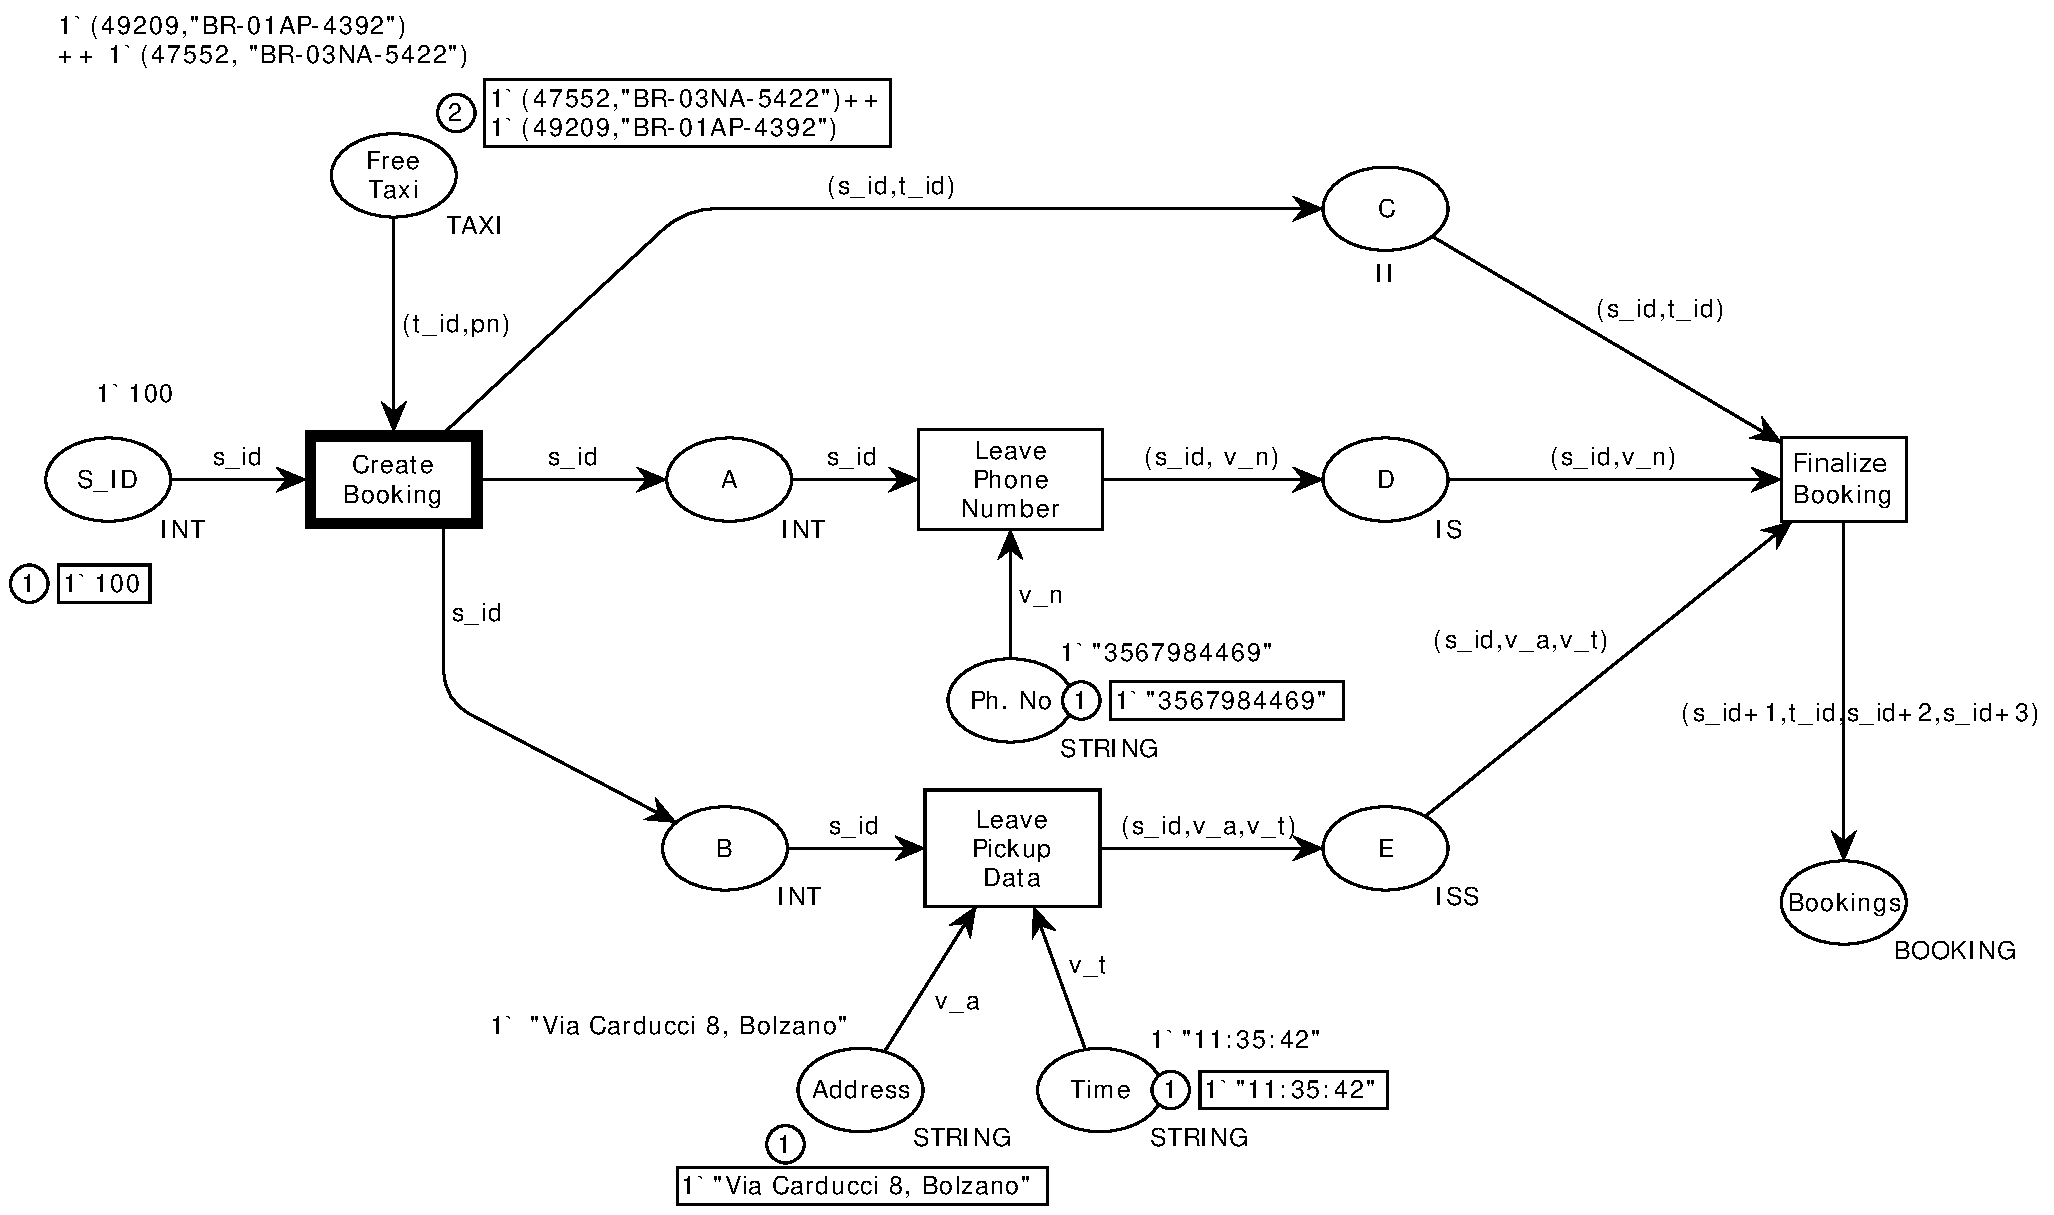
\includegraphics[scale = 0.4]{CPN_Taxi_Booking_simple.pdf}
	\caption{Revised CPN model showing a state for taxi booking example}
	\label{fig:CPN_Taxi_Booking_simple}
\end{figure}

\begin{figure}
	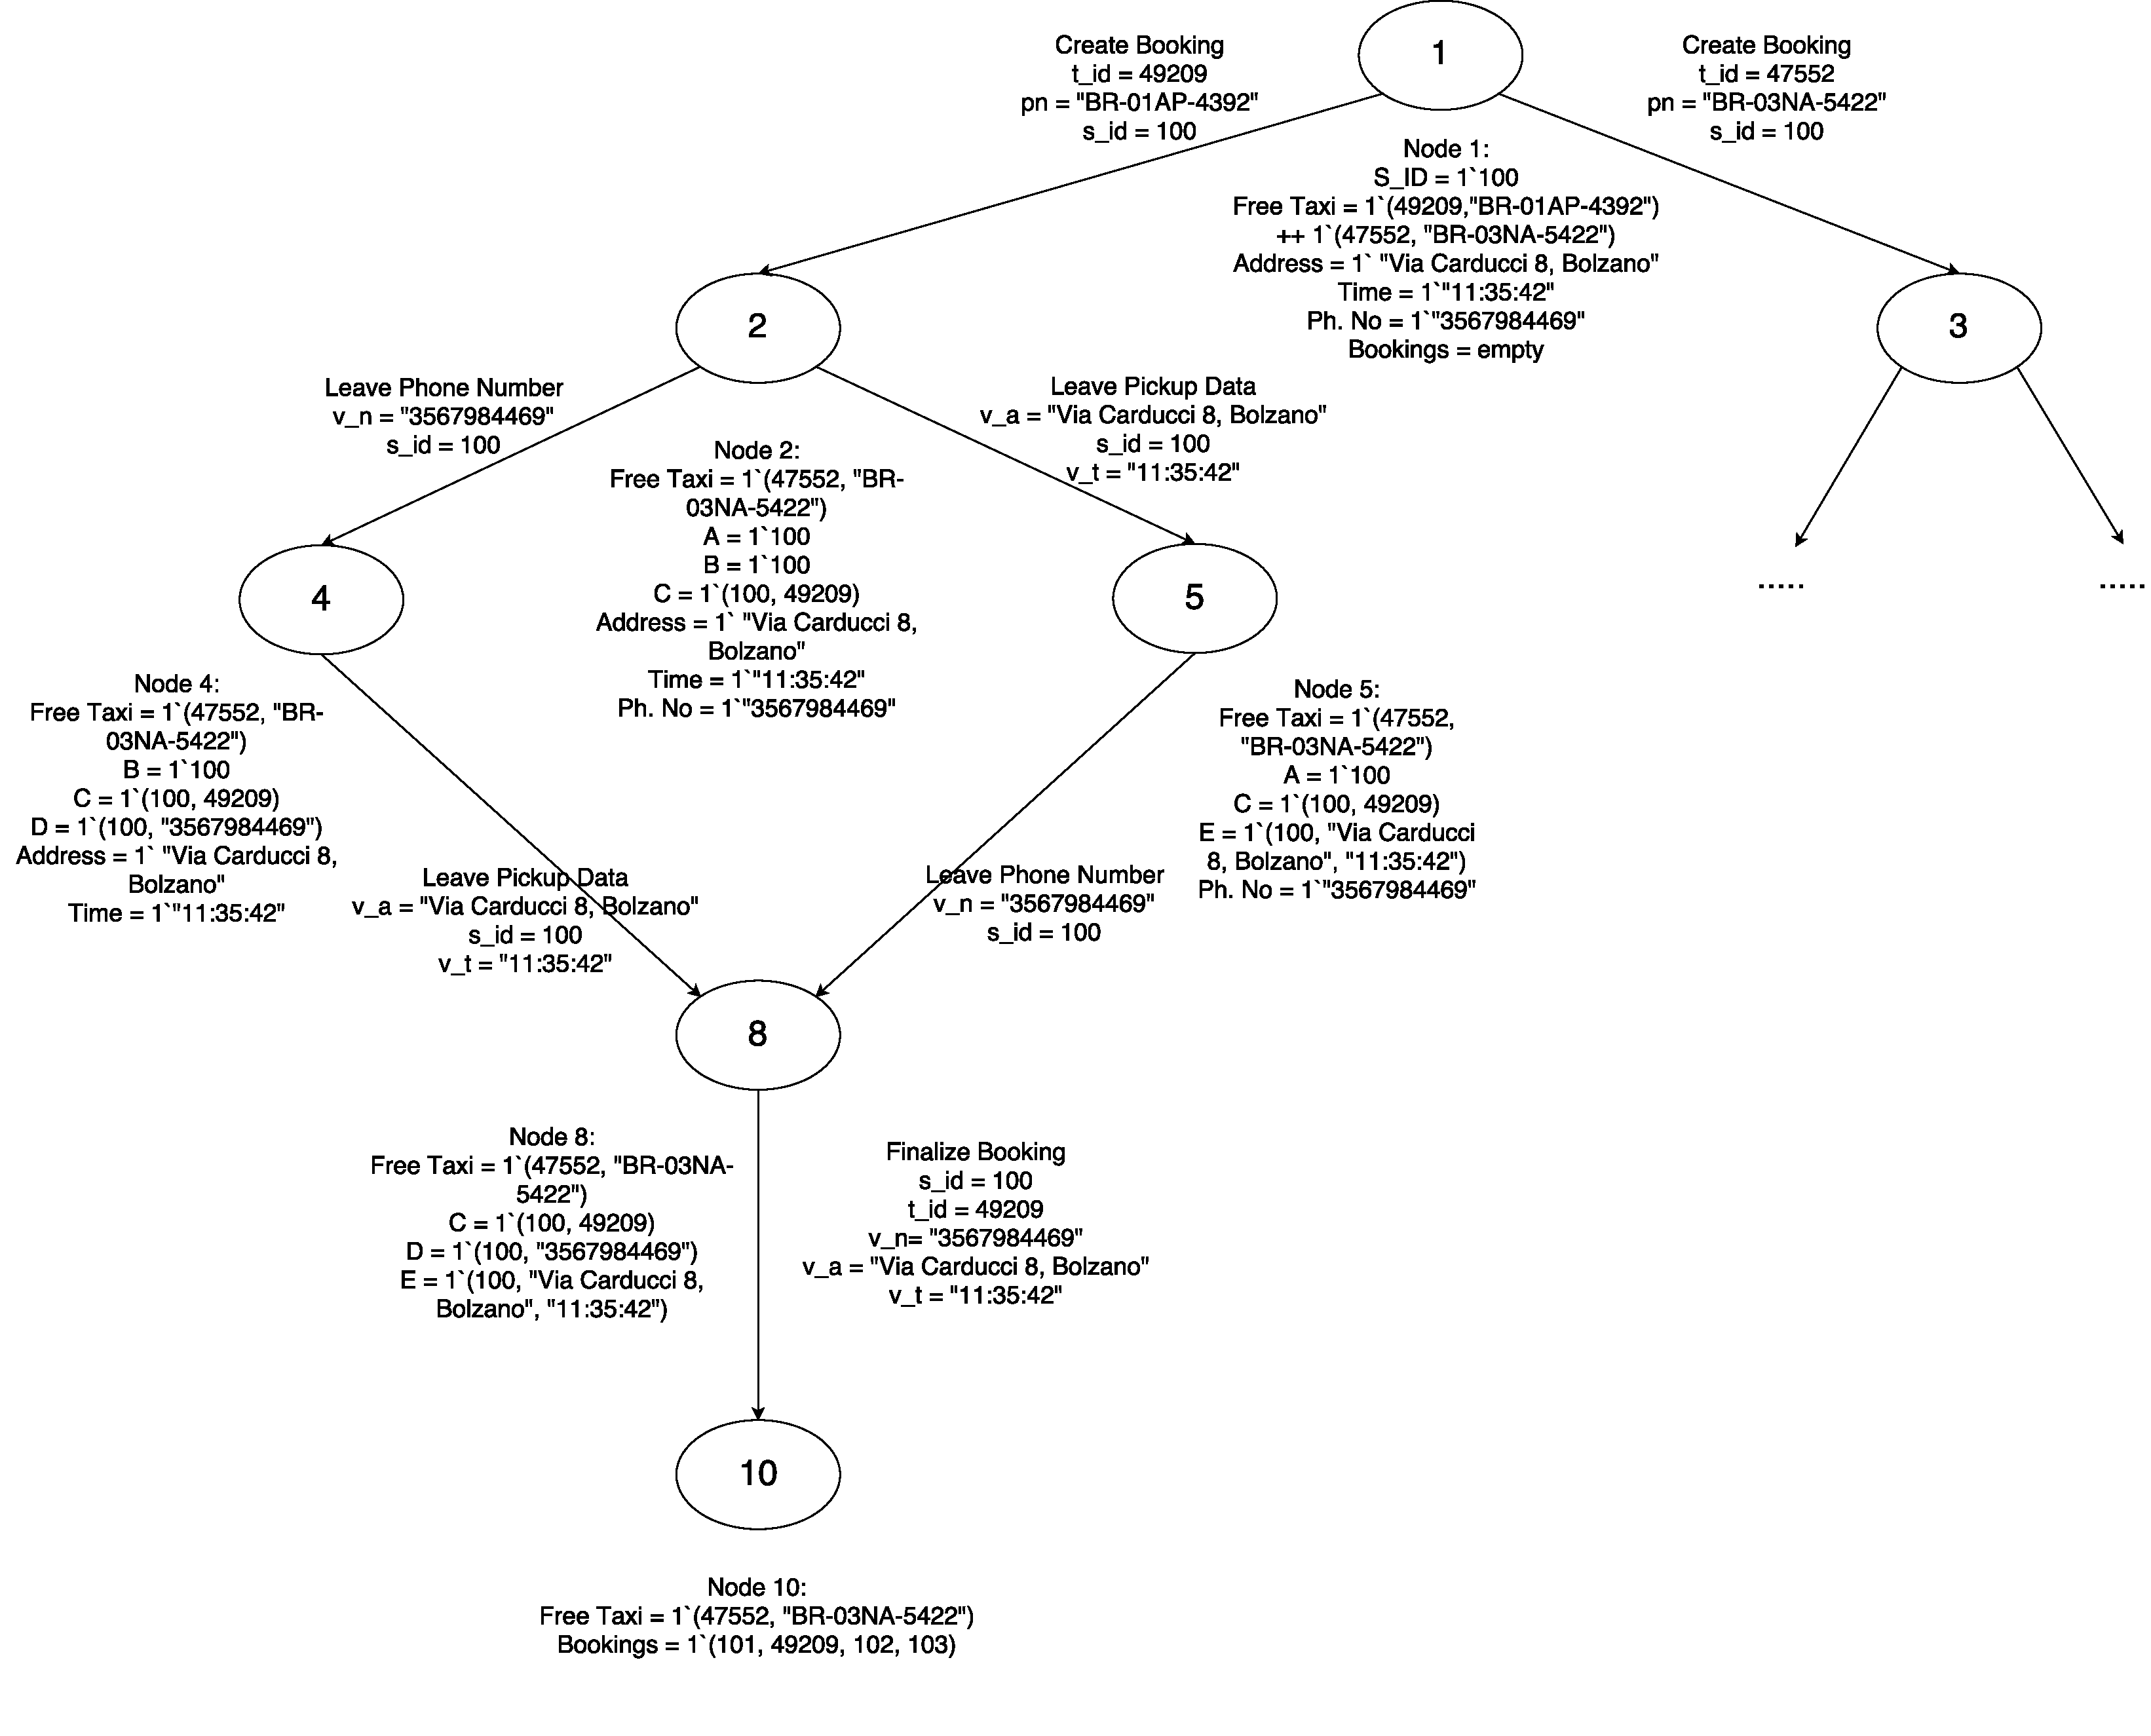
\includegraphics[scale = 0.21]{CPN_Taxi_Booking_State_Space.pdf}
	\caption{State Space for CPN model in Figure \ref{fig:CPN_Taxi_Booking_simple}}
	\label{fig:CPN_State_Space}
\end{figure}
